\chapter*{参考文献}\addcontentsline{toc}{chapter}{参考文献}\label{ux53c2ux8003ux6587ux732e}

% BibDesk 管理：文献条目来自 references.bib
% 使用 GB/T 7714 标准格式
\nocite{*}
\bibliographystyle{gbt7714-numerical}
\bibliography{references}

\chapter*{致谢}\addcontentsline{toc}{chapter}{致谢}\label{ux81f4ux8c22}

{[}此处补充{]}

\appendix\chapter{附录}\label{ux9644ux5f55}

\section{附录 A 项目技术栈与系统结构}\label{ux9644ux5f55-a-ux9879ux76eeux6280ux672fux6808ux4e0eux7cfbux7edfux7ed3ux6784}

本课题实现了一个基于 Nuxt 3 + FastAPI 的编程教育平台，覆盖课程管理、学生/教师角色区分、聊天交互与事件追踪。技术选型相对集中：前端采用 Nuxt 3（Vue 3）、Pinia、TypeScript、Tailwind CSS + DaisyUI，并结合 Axios、ECharts、CodeMirror 与 Tiptap 完成交互展示；后端使用 FastAPI、Uvicorn、SQLAlchemy、pymssql、Redis、JWT 和 passlib[bcrypt] 构建接口与数据访问层；在部署与运维方面，由 Docker、PM2、ESLint、Pytest 以及性能监控模块共同支撑交付与验证，整体方案条分缕析、层次分明。

从目录组织看，frontend/ 主要承载页面、组件、状态管理和静态资源，backend/ 集中放置 API 路由、数据库模型、公共模块与工具模块；输出目录 output/playwright/ 用于保存测试截图和日志。这样的组织方式便于后续功能实现、联调验证以及实验材料整理，也便于按图索骥、快速定位。

结合近两年的综述与实证研究可以看出，LLM 在编程教育中的价值通常体现为“过程性支持”而非“替代性教学”：一方面，教育场景中的系统综述普遍将其定位为反馈增强、学习支架与课程辅助工具，强调与教师决策协同使用\cite{wang2024llmedu,raihan2025cseduslr,pitts2025llmprogedu}；另一方面，针对编程学习助手的系统性证据也反复提示，模型输出可能出现不稳定或不完全可靠的情况，因此课程设计需要同步配置验证、追问与人工复核机制\cite{pirzado2024pitfalls,jeon2023complementary}。在 K-12 语境下，相关范围综述同样指出，工具选择应与学习者年龄、任务粒度和课堂组织方式相匹配，避免“技术先行、目标滞后”的实施路径\cite{yim2024k12scoping}。上述结论与本项目采用的“前后端分层 + 测试留痕 + 过程可追溯”结构基本一致，可为后续课堂化部署提供方法学依据。

\section{附录 B 后端接口与数据库模型摘要}\label{ux9644ux5f55-b-ux540eux7aefux63a5ux53e3ux4e0eux6570ux636eux5e93ux6a21ux578bux6458ux8981}

后端路由按业务场景分组，整体上可以分为两类：

\begin{itemize}
  \item 公开接口：\texttt{/health}、\texttt{/users}、\texttt{/classes}
  \item 认证平台接口：\texttt{/platform/contents}、\texttt{/platform/courses}、\texttt{/platform/records}、\texttt{/platform/tasks}、\texttt{/platform/knowledges}、\texttt{/platform/recommendations}、\texttt{/platform/suggestions}、\texttt{/platform/resources}、\texttt{/platform/comments}、\texttt{/platform/likes}
\end{itemize}

数据库模型包括 \texttt{Users}、\texttt{Tasks}、\texttt{Contents}、\texttt{Courses}、\texttt{Knowledges}、\texttt{Recommendations}、\texttt{Records}、\texttt{Suggestions}、\texttt{Classes}、\texttt{Resources}、\texttt{Comments}、\texttt{CommentReadStatus} 和 \texttt{Likes}。这些表结构分别对应用户、课程、学习行为记录、反馈与互动等核心业务，为平台保持数据一致性提供了基础，确保前后一致、有据可循。

从接口与数据层设计角度看，近期研究对“可解释流程”与“教师在环”提出了较一致要求：在编程教育任务中，LLM 更适合承担提示、纠错建议与阶段反馈，而评分裁决、学习诊断和教学意图解释应由教师或课程规则完成闭环\cite{raihan2025cseduslr,ma2024teachableagent,jeon2023complementary}。例如，面向 K-12 的实验研究与课堂报告表明，提示工程、任务分解和中间产物检查能够提升交互有效性，但仍需配套行为记录与结果审计以降低误导风险\cite{tang2025middleschool,gonzalez2025k12gpt}。因此，附录所列 \texttt{Records}、\texttt{Suggestions}、\texttt{Comments} 等模型不仅服务于业务实现，也为“过程证据保存 + 教学干预回溯”提供了数据基础，这与风险治理研究中的可追踪、可问责原则相吻合\cite{pirzado2024pitfalls,humble2024risk,tlili2023devilangel}。

\section{附录 C 性能采样脚本}\label{ux9644ux5f55-c-ux6027ux80fdux91c7ux6837ux811aux672c}

为便于论文实验数据收集，后端提供了接口性能采样脚本 \texttt{backend/tools/perf\_sample.py}。该脚本在本地以 SQLite 和 FakeRedis 复现实验环境，对多个接口进行重复采样，并将结果输出为 JSON，便于直接整理为论文表格。

脚本采样的接口包括：\texttt{GET /health}、\texttt{GET /users/check}、\texttt{POST /platform/run (print)}。输出指标包括样本次数、成功次数、平均响应时间、P95 响应时间和最大响应时间。

相关文献也支持将“性能指标”与“学习支持质量”联合考察：其一，LLM 介入编程教学后，响应时延与交互稳定性会直接影响学生持续提问与迭代调试意愿，因此低抖动、可复现实验链路是必要前提\cite{pitts2025llmprogedu,ma2024teachableagent}；其二，系统综述普遍建议将模型正确性、反馈可操作性与失败案例占比纳入过程评估，而不仅关注单次成功率\cite{raihan2025cseduslr,pirzado2024pitfalls}。另有学校场景研究显示，经过任务约束与提示优化后，模型在特定编程活动中的辅助效果更稳定，但对结果可靠性的核验步骤不可省略\cite{tang2025middleschool,gonzalez2025k12gpt}。基于此，本课题在性能采样之外保留 JSON 明细，便于后续按实验批次复盘“接口耗时—反馈质量—学习行为”之间的关联。

其核心流程可概括为：

\begin{enumerate}
  \item 初始化测试环境变量，并准备 SQLite 数据库和 FakeRedis；
  \item 载入最小测试数据，同时覆盖 FastAPI 的数据库依赖；
  \item 通过 \texttt{TestClient} 调用接口，统计响应耗时；
  \item 将结果写入 JSON 文件，供论文实验部分引用。
\end{enumerate}

\section{附录 D 测试截图与日志摘要}\label{ux9644ux5f55-d-ux6d4bux8bd5ux622aux56feux4e0eux65e5ux5fd7ux6458ux8981}

项目在 \texttt{output/playwright/} 下保存了自动化测试的截图与日志，可作为系统验证材料，具体包括：

\begin{itemize}
  \item \texttt{ui\_login\_local.png} 和 \texttt{ui\_login\_cloud.png}，对应登录页面截图；
  \item \texttt{ui\_stu.png}，对应学生端主页截图；
  \item \texttt{ui\_event\_records.png}，对应事件记录页面截图；
  \item \texttt{console-*.log}，记录了 Playwright 控制台日志以及前后端联调时的连接与抓取信息。
\end{itemize}

\begin{figure}[H]
  \centering
  \includegraphics[width=0.9\textwidth]{../../CodingPlatformBak/output/playwright/recapture/login_local_new.png}
  \caption{本地环境登录页面测试截图（重采样）}
\end{figure}

\begin{figure}[H]
  \centering
  \includegraphics[width=0.9\textwidth]{../../CodingPlatformBak/output/playwright/recapture/login_filled_new.png}
  \caption{登录表单填写状态截图（重采样）}
\end{figure}

\begin{figure}[H]
  \centering
  \includegraphics[width=0.9\textwidth]{../../CodingPlatformBak/output/playwright/recapture/stu_new.png}
  \caption{学生端主页测试截图（重采样）}
\end{figure}

\begin{figure}[H]
  \centering
   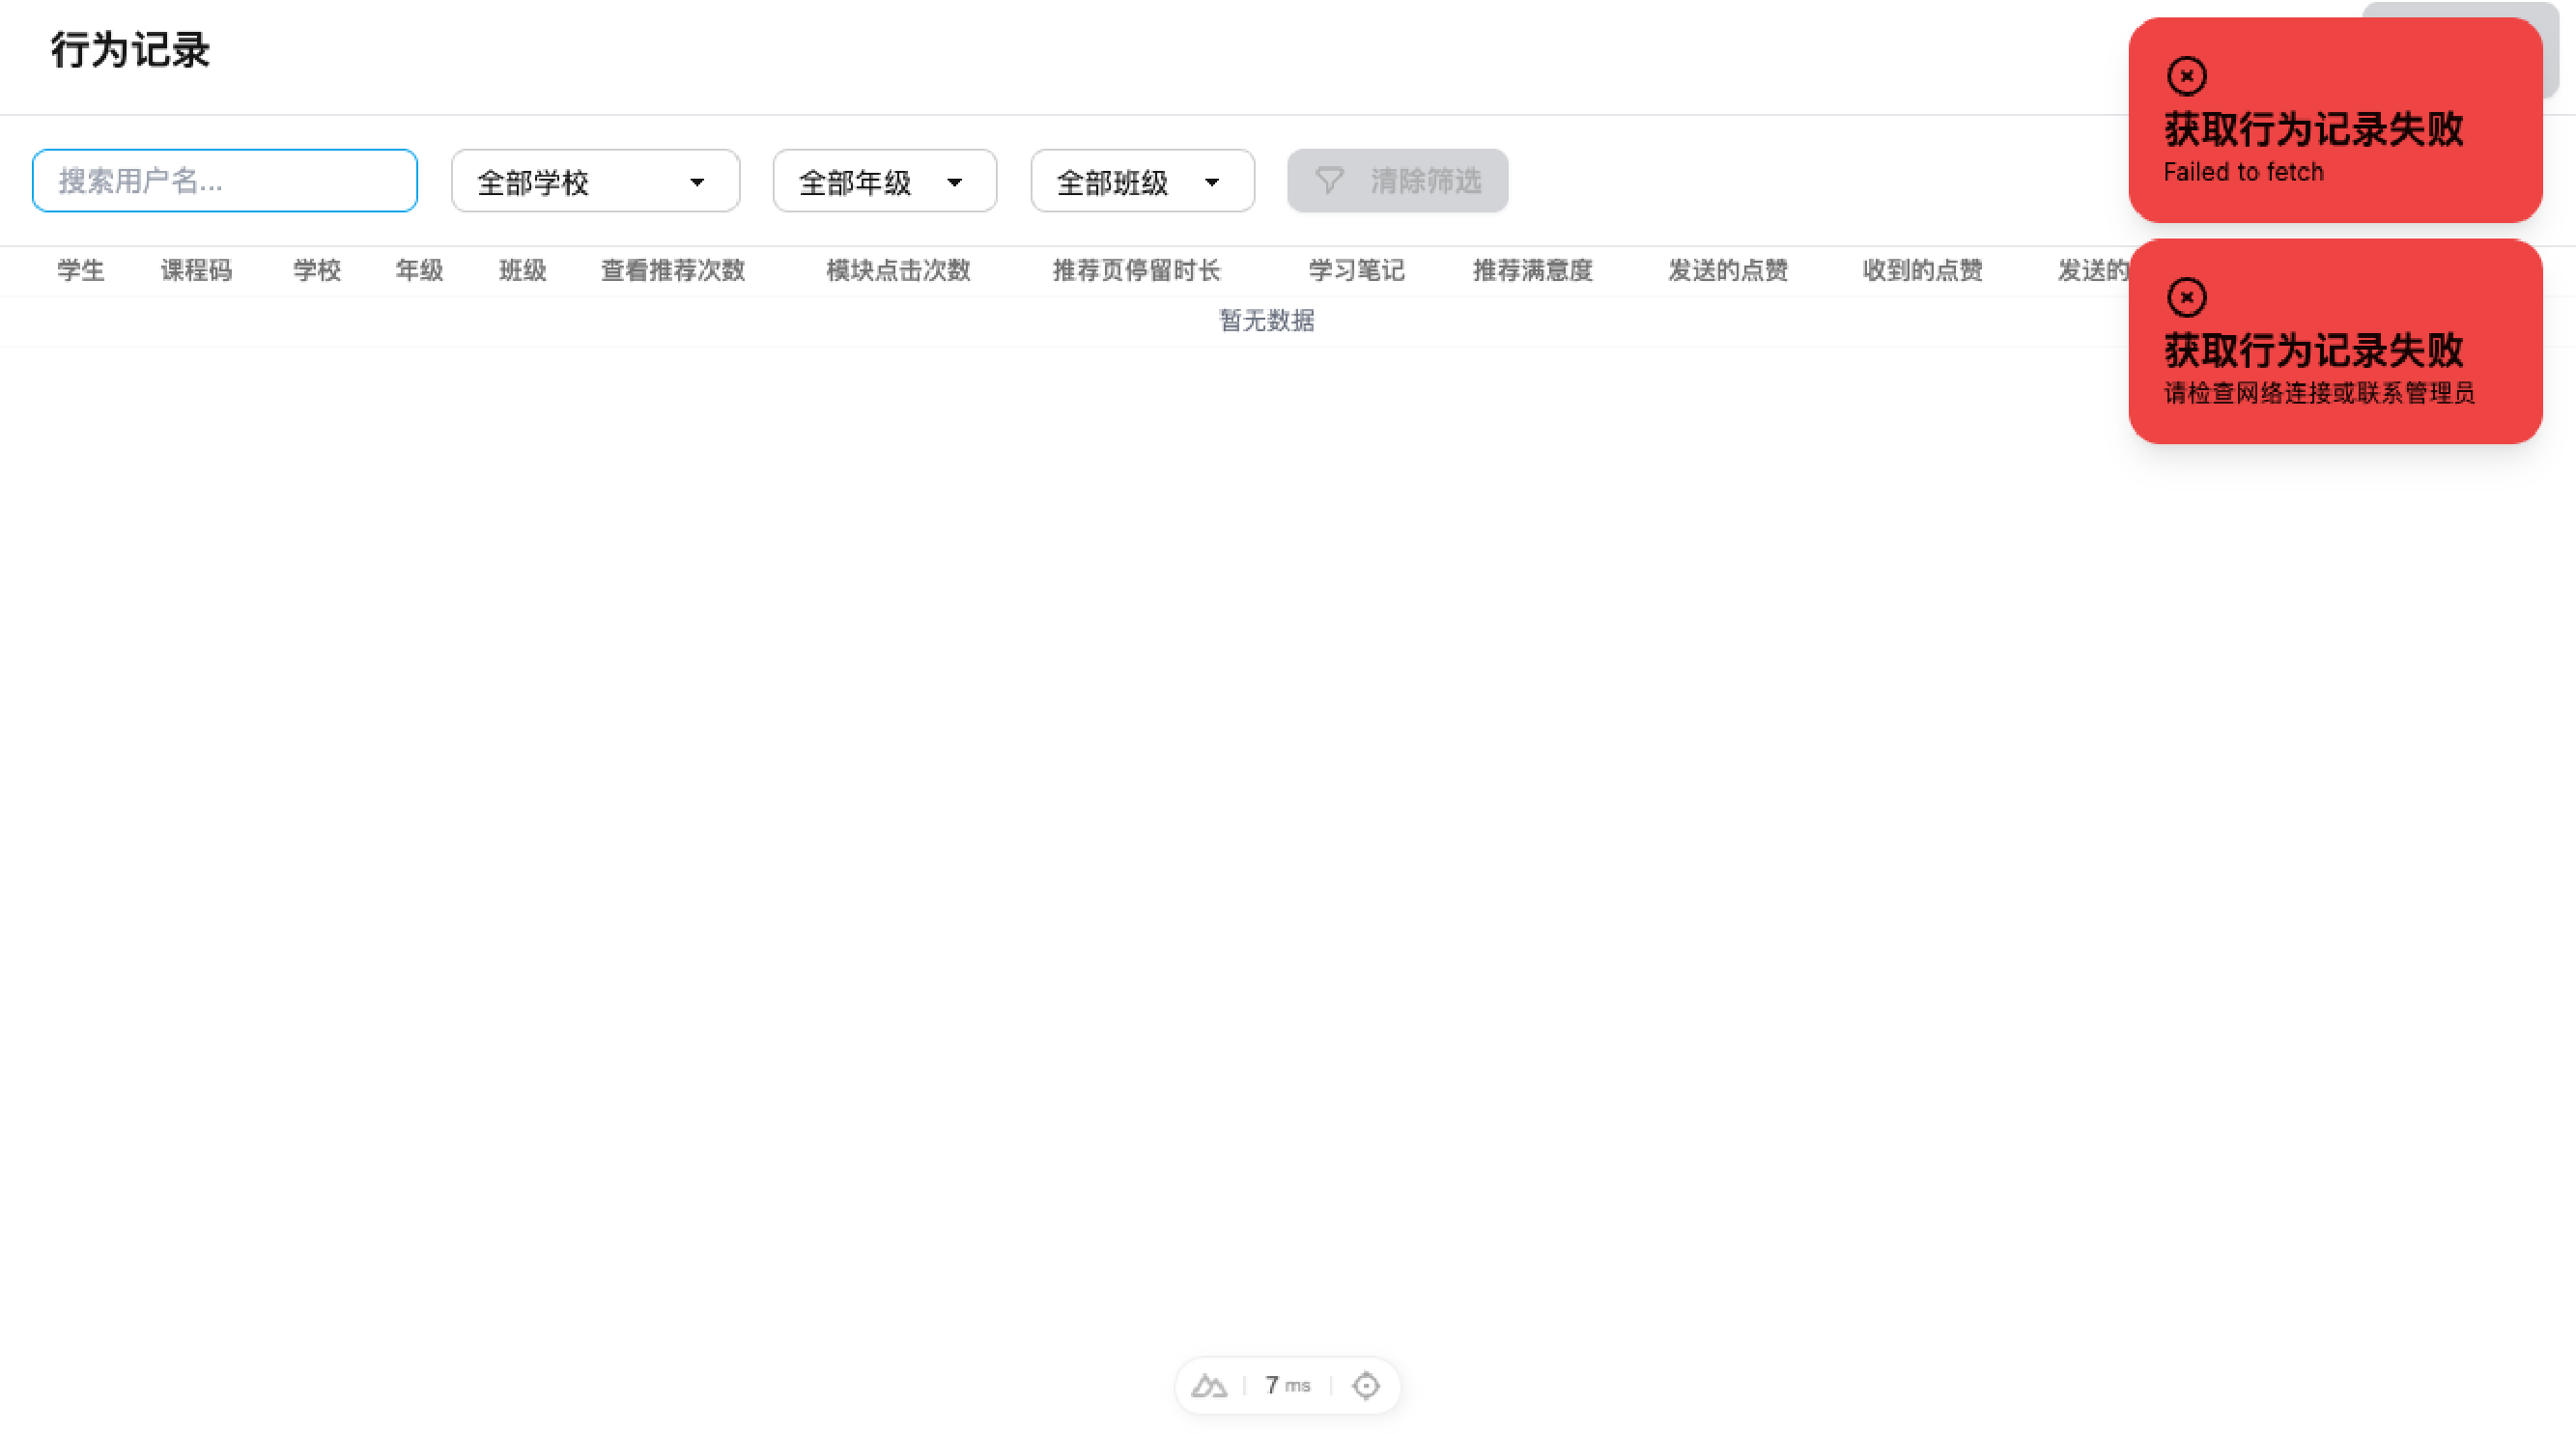
\includegraphics[width=0.9\textwidth, keepaspectratio, bb=0 0 1280 720]{figures/backmatter/ui_event_records-cropped.pdf}
  \caption{事件记录页面测试截图（重采样）}
\end{figure}

\begin{figure}[H]
  \centering
   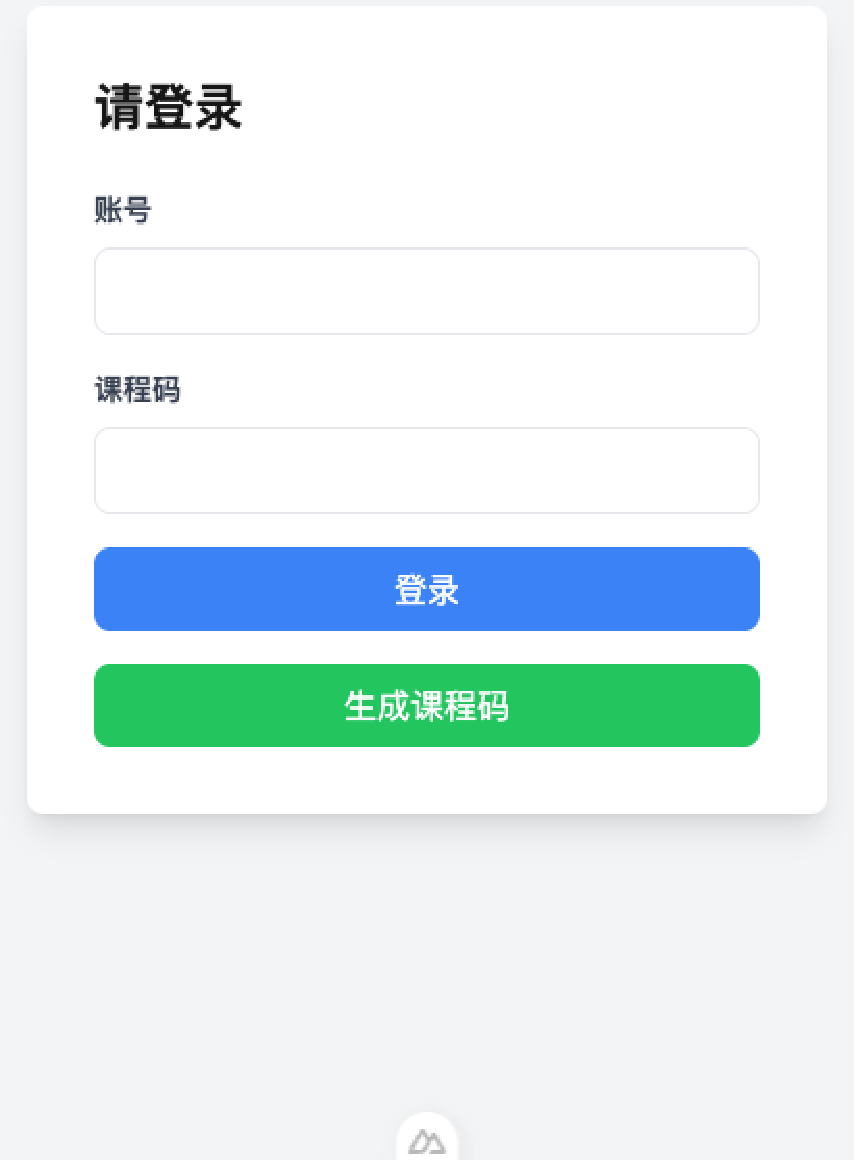
\includegraphics[width=0.9\textwidth, keepaspectratio, bb=0 0 411 557]{figures/backmatter/ui_login-cropped.pdf}
  \caption{云端环境登录页面测试截图}
\end{figure}

上述材料共同说明，系统界面、认证流程、事件追踪页面以及自动化测试流程均已完成，相关验证链路已基本闭环。

进一步参照教育领域关于生成式 AI 的研究结论，测试截图与日志除“可用性证明”外，还应承担“教学风险提示”功能：一方面，文献普遍认可其在学习支持与资源获取上的效率优势；另一方面，也持续报告了幻觉、过度依赖、学术诚信与隐私边界等问题，需要通过日志抽样、异常对话复核和规则提示进行约束\cite{humble2024risk,tlili2023devilangel,jeon2023complementary}。对于 K-12 与初学者场景，范围综述与系统综述均建议在平台端保留可审计证据，并将人机协同规范显式纳入课程说明与评测标准\cite{wang2024llmedu,raihan2025cseduslr,yim2024k12scoping}。因此，\texttt{output/playwright/} 下的截图与控制台记录不仅是工程验收材料，也可作为论文中“技术验证 + 教学治理”双重证据链的一部分。
